% This is samplepaper.tex, a sample chapter demonstrating the
% LLNCS macro package for Springer Computer Science proceedings;
% Version 2.20 of 2017/10/04
%
\documentclass[runningheads]{llncs}
%
\usepackage{graphicx}
% Used for displaying a sample figure. If possible, figure files should
% be included in EPS format.
%
% If you use the hyperref package, please uncomment the following line
% to display URLs in blue roman font according to Springer's eBook style:
% \renewcommand\UrlFont{\color{blue}\rmfamily}
\begin{document}

\title{Factorisation matricielle non-n\'egative et classification d'images}

\author{MOHAMED BEN HAMDOUNE\inst{1} et YANNIS TANNIER\inst{1}}

\authorrunning{M. Ben Hamdoune et al.}

\markboth{M. Ben Hamdoune, Y. Tannier}{Factorisation matricielle non-n\'egative et classification d'images}

\institute{Universit\'e Paris-Descartes, 12 Rue de l'\'Ecole de M\'edecine, 75006 Paris, France,
\email{mohamed.ben\_hamdoune@etu.parisdescartes.fr}\\ 
\\
\email{yannis.tannier@etu.parisdescartes.fr}\\
\url{https://www.univ-paris5.fr/}}
%
\maketitle              % typeset the header of the contribution
%
\begin{abstract}
La classification automatique ou $clustering$ consiste \`a partionner un ensemble d'objets (instances) d\'ecrits par un ensemble de variables en groupes (classes) homog\`enes. Avec l'av\`enement du $Big Data$ et de la science des donn\'ees, le clustering est devenu une t\^ache encore tr\`es importante dans divers domaines dont l'imagerie. Les images sont des donn\'ees tr\`es r\'epandues notamment sur le web et les r\'eseaux sociaux (Instagram, Pinterest, Flickr, Google,etc...).Le but sera de proposer un syst\'eme de classification pour des images provenant de divers bases de donn\'ees (photos, peintures, bandes dessin\'es, etc). La factorisation matricielle non-n\'egative permet d'approximer une matrice de donn\'ees positive par le produit de deux matrices de dimensions inf\'erieures et positives. Par sa simplicit\'e, cette m\'ethode est devenue populaire et est utilis\'ee \`a la fois dans la r\'eduction de la dimension et \'egalement dans la classification automatique (clustering) en un nombre de classes $k$ fix\'e par l'utilisateur. 
\keywords{Apprentissage Non Supervis\'e, Spherical K-means, K-means, R, NMF, Python, Scikit-Learn, Nimfa, NmfGpu4R, Cuda}
\end{abstract}
%
\section{Introduction}
\subsection{La factorisation matricelle non-n\'egative}

Cette section donne une d\'efinition formelle des probl\`emes de factorisation matricielle non-n\'egative et d\'efinit les notations utilis\'ees dans le cadre de ce TER (\textbf{Travail d'\'etudes et de recherches}).

Soit $X$ une matrice non-n\'egative $n \times p$, (i.e avec $x_{ij} \geq 0$,
tel que $X \geq 0$), et $r > 0$ un entier positif. 
La factorisation matricielle non-n\'egative (\textbf{NMF}) consiste \`a trouver une approximation
\begin{equation}
X \approx W H\ , \label{NMFstd}
\end{equation} o\`u $W, H$ sont $n\times r$ et $r \times p$ matrices non-n\'egativs respectivement.
En pratique, le rang de factorisation $r$ est souvent choisis de tel sorte que $r \ll \min(n, p)$. 
L'objectif derrière ce choix est de r\'esumer et diviser l'information contenue dans $X$ en facteurs $r$: les colonnes de $W$.

Selon le domaine d'application, ces facteurs ont des noms diff\'erents: images de base, m\'etag\`enes, signaux source. Dans cette vignette, nous utilisons de mani\`ere \'equivalente et alternative les termes \emph{base matrice} ou \emph{metag\`enes} pour faire r\'ef\'erence \`a la matrice $W$, et \emph{matrice de coefficients de m\'elange} et \emph{profils d'expression de m\'etag\`ene} pour se r\'ef\'erer \'a la matrice $H$.
La principale approche du \textbf{NMF} consiste \`a estimer les matrices $W$ et $H$ comme un minimum local:
\begin{equation}
\min_{W, H \geq 0}\ \underbrace{[D(X, WH) + R(W, H)]}_{=F(W,H)} \label{nmf_min}
\end{equation}
o\`u

\begin{itemize}
\item $D$ est une fonction de perte qui mesure la qualit\'e de l'approximation.
Les fonctions de perte communes sont bas\'ees soit sur la distance de Frobenius
$$D: A,B\mapsto \frac{Tr(AB^t)}{2} = \frac{1}{2} \sum_{ij} (a_{ij} - b_{ij})^2,$$
ou la divergence Kullback-Leibler.
$$D: A,B\mapsto KL(A||B) = \sum_{i,j} a_{ij} \log \frac{a_{ij}}{b_{ij}} - a_{ij} + b_{ij}.$$
\item $ R $ est une fonction de r\'egularisation facultative, d\'efinie pour appliquer
les propri\'et\'es sur les matrices $ W $ et $ H $, telles que la $smoothness$ ou la $sparsit\'e$ \cite{Cichocki2008}.
\end{itemize}

\paragraph{Sample Heading (Fourth Level)}
The contribution should contain no more than four levels of
headings. Table~\ref{tab1} gives a summary of all heading levels.

\subsection{Les m\'ethodes de partitionnement}
on parle de clustering

\section{Construction de la matrice num\'erique}

\section{Estimation du rang de la factorisation}

\section{M\'ethodes d'initialisation}

\section{Classification}

\section{Conclusion}

Un param\'`etre critique dans la \textbf{NMF} est le rang de la factorisation $r$.
Il d\'efinit le nombre de variables utilis\'es pour approcher la matrice cible.
\'Etant donn\'e une m\'ethode \textbf{NMF} et la matrice cible, une façon courante de d\'ecider de $r $ est d'essayer diff\'erentes valeurs, de calculer une mesure de qualit\'e des r\'esultats et de choisir la meilleure valeur en fonction de ces critères de qualit\'e.

Several approaches have then been proposed to choose the optimal value of $r$.
For example, \cite{Brunet2004} proposed to take the first value of $r$ for which the cophenetic coefficient starts decreasing, \cite{Hutchins2008} suggested to choose the first value where the RSS curve presents an inflection point, and \cite{Frigyesi2008} considered the smallest value at which the decrease in the RSS is lower than the decrease of the RSS obtained from random data.

Le package \textbf{NMF} provides functions to help implement such procedures and plot the relevant quality measures.
Note that this can be a lengthy computation, depending on the data size.
Whereas the standard NMF procedure usually involves several hundreds of random initialization, performing 30-50 runs is considered sufficient to get a robust estimate of the factorization rank \cite{Brunet2004, Hutchins2008}.
For performance reason, we perform here only 10 runs for each value of the rank.

The result is a S3 object of class NMF.rank, that contains a data.frame with the quality measures in column, and the values of $r$ in row.
It also contains a list of the consensus matrix for each value of $r$.

All the measures can be plotted at once with the method, and the function generates heatmaps of the consensus matrix for each value of the rank.
In the context of class discovery, it is useful to see if the clusters obtained correspond to known classes.
This is why in the particular case of the Golub dataset, we added annotation tracks for the two covariates available ('Cell' and 'ALL.AML').
Since we removed the variable 'Sample' in the preliminaries, these are the only variables in the phenotypic data.frame embedded within the ExpressionSet object, and we can simply pass the whole object to argument annCol.
One can see that at rank 2, the clusters correspond to the ALL and AML samples respectively, while rank 3 separates AML from ALL/T-cell and ALL/B-cell\footnote{Remember that the plots shown in come from only 10 runs, using the 200 first genes in the dataset, which explains the somewhat not so clean clusters.
The results are in fact much cleaner when using the full dataset.}.

\begin{figure}
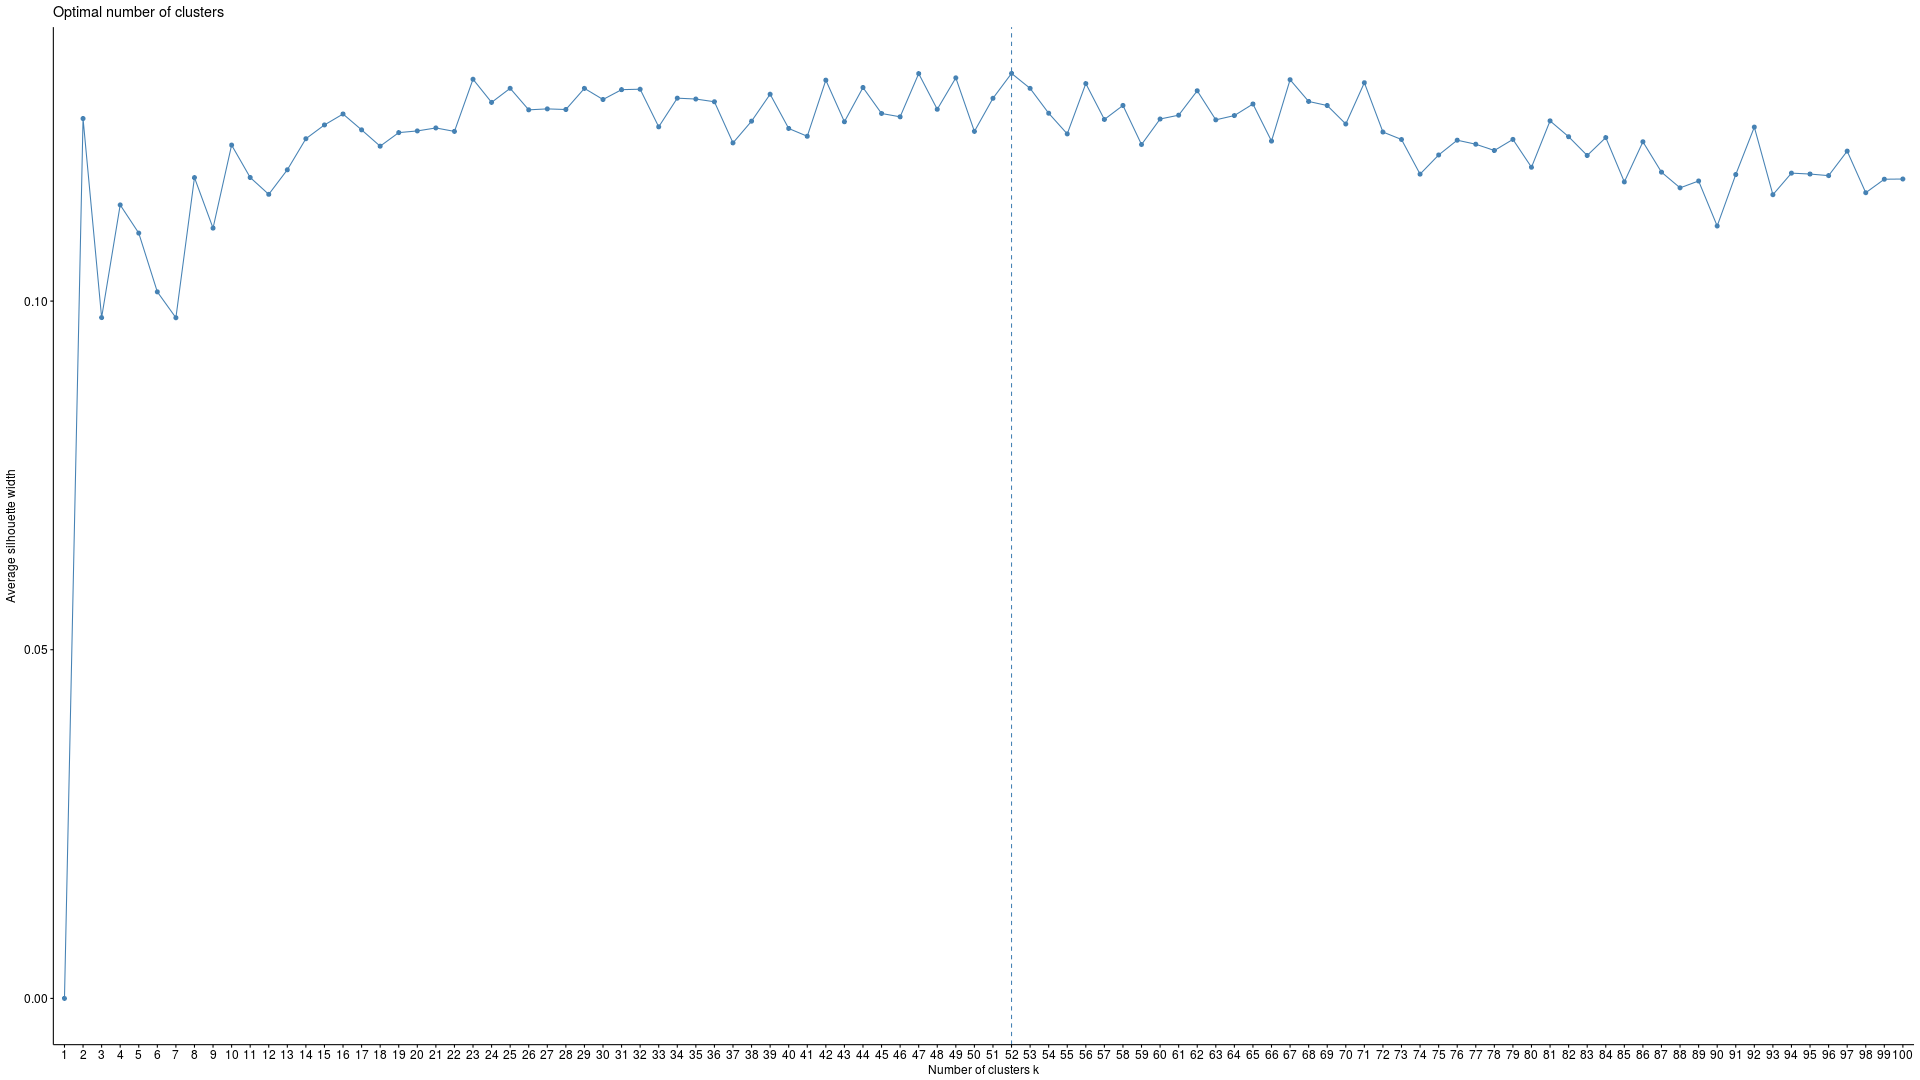
\includegraphics[width=\textwidth]{x16_k_greyscale.png}
\caption{La largeur moyenne de la silhouette en utilisant K-means pour un intervalle de 1 \'a 100, le nombre de clust optimal est 51.} \label{fig1}
\end{figure}

\begin{figure}
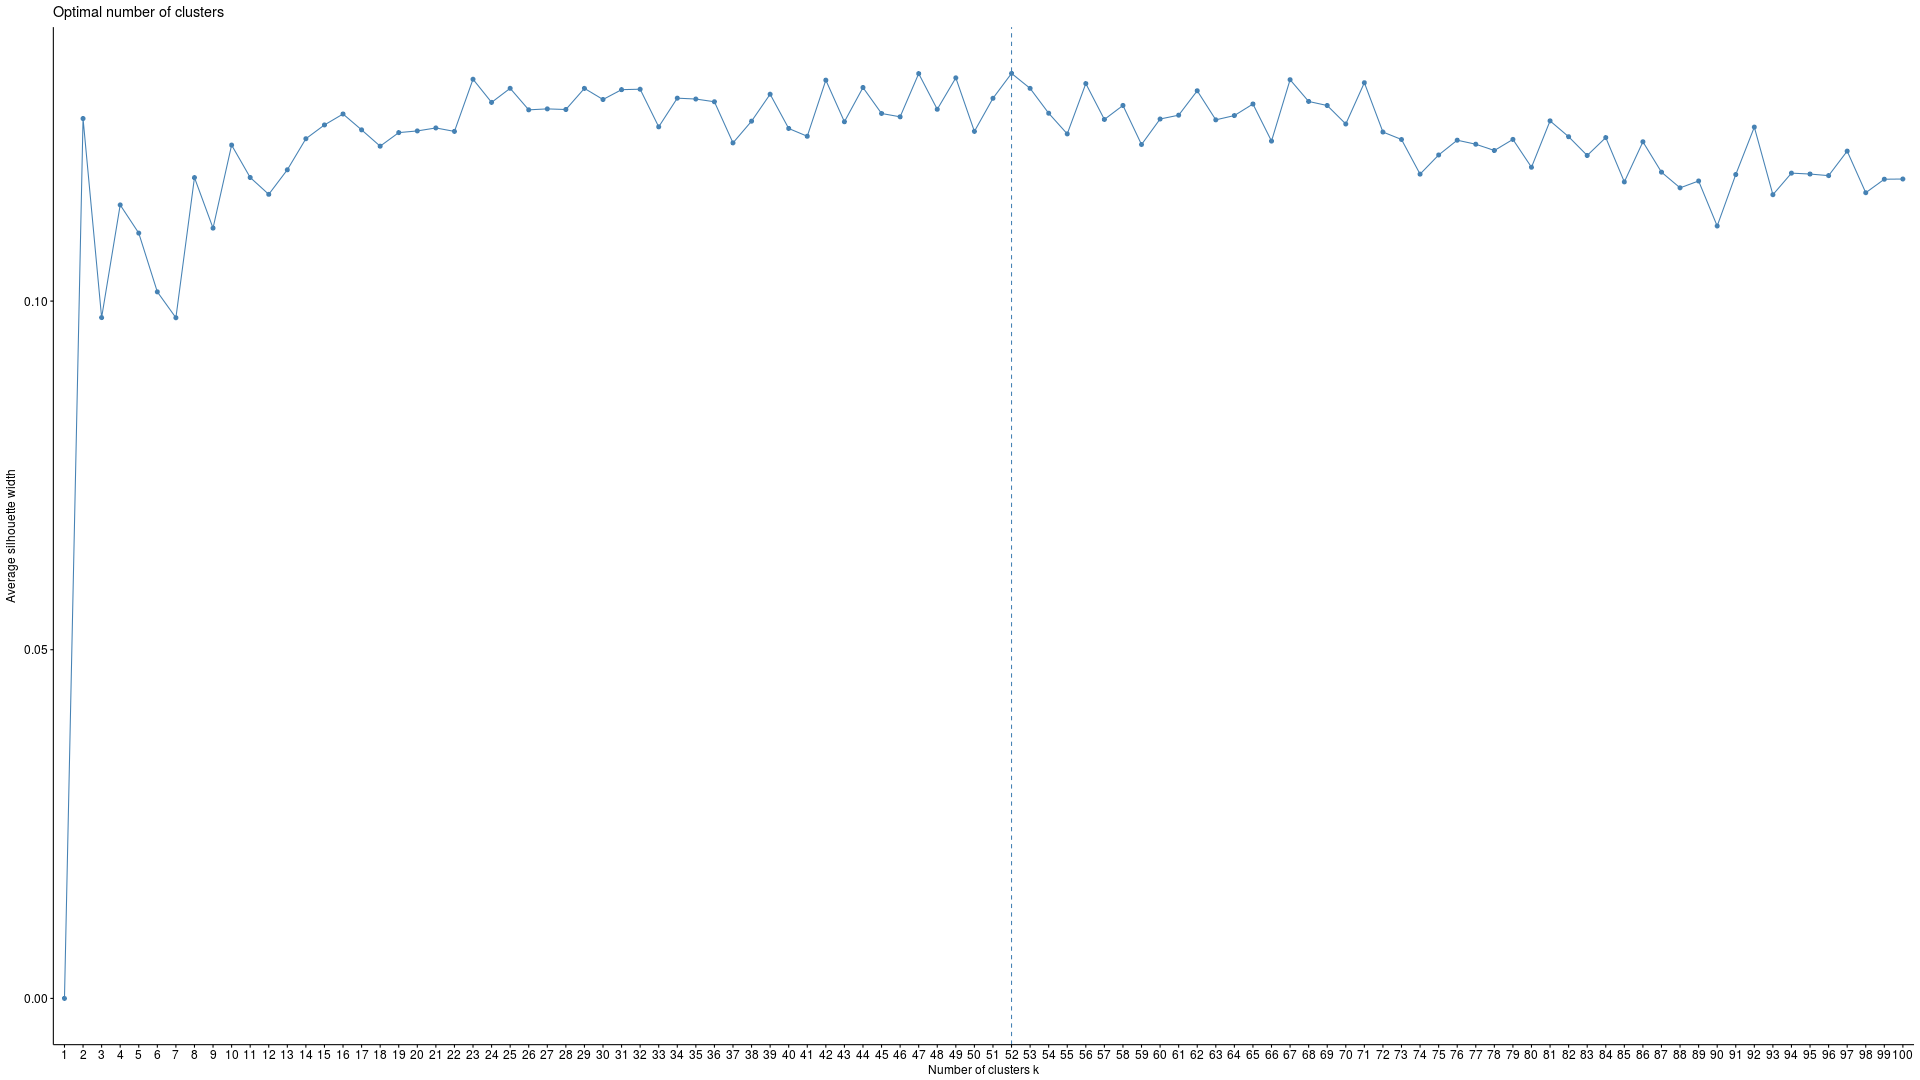
\includegraphics[width=\textwidth]{x16_k_greyscale.png}
\caption{La largeur moyenne de la silhouette en utilisant K-means pour un intervalle de 1 \`a 100, le nombre de clust optimal est 52 pour des blocs 16x16 avec un filtre gris.} \label{fig2}
\end{figure}

\begin{figure}
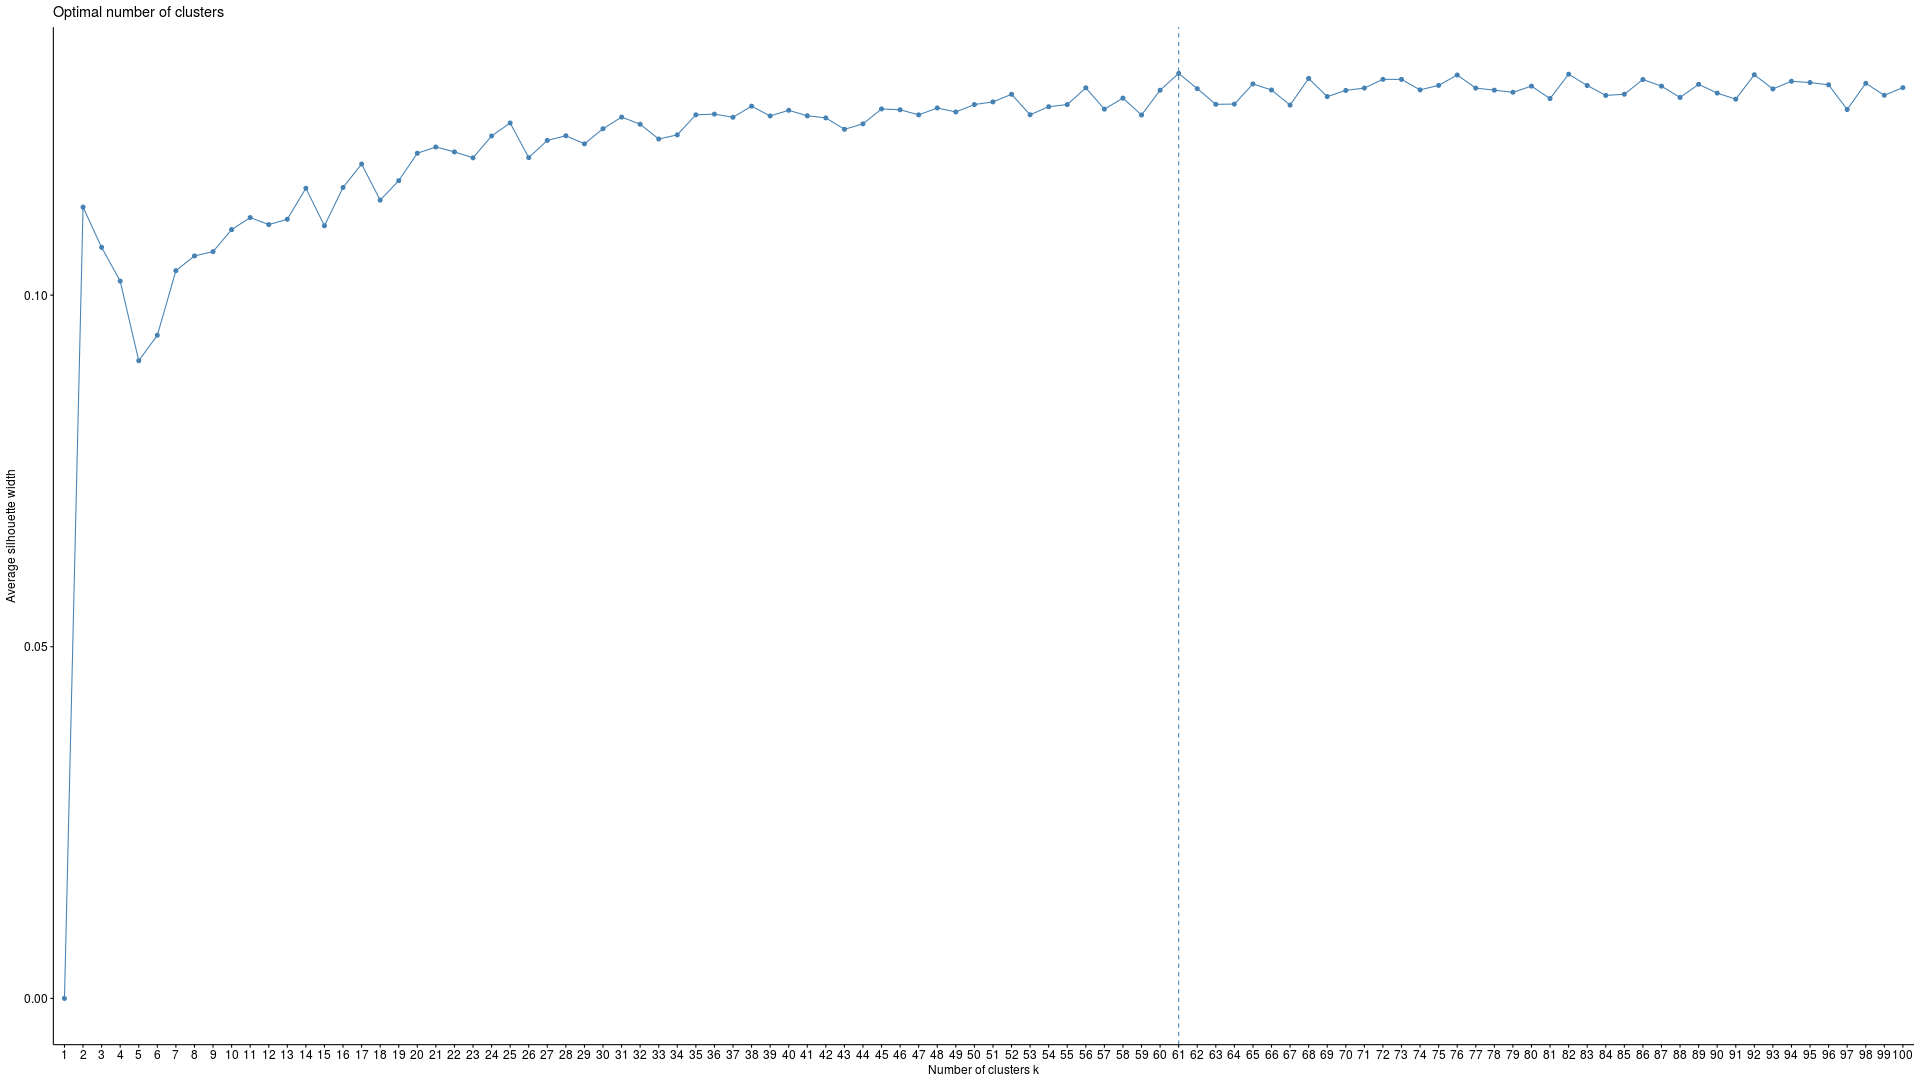
\includegraphics[width=\textwidth]{x32_k_greyscale.png}
\caption{La largeur moyenne de la silhouette en utilisant K-means pour un intervalle de 1 \`a 100, le nombre de clust optimal est 61 pour des blocs 32x32 avec un filtre gris.} \label{fig3}
\end{figure}

\begin{figure}
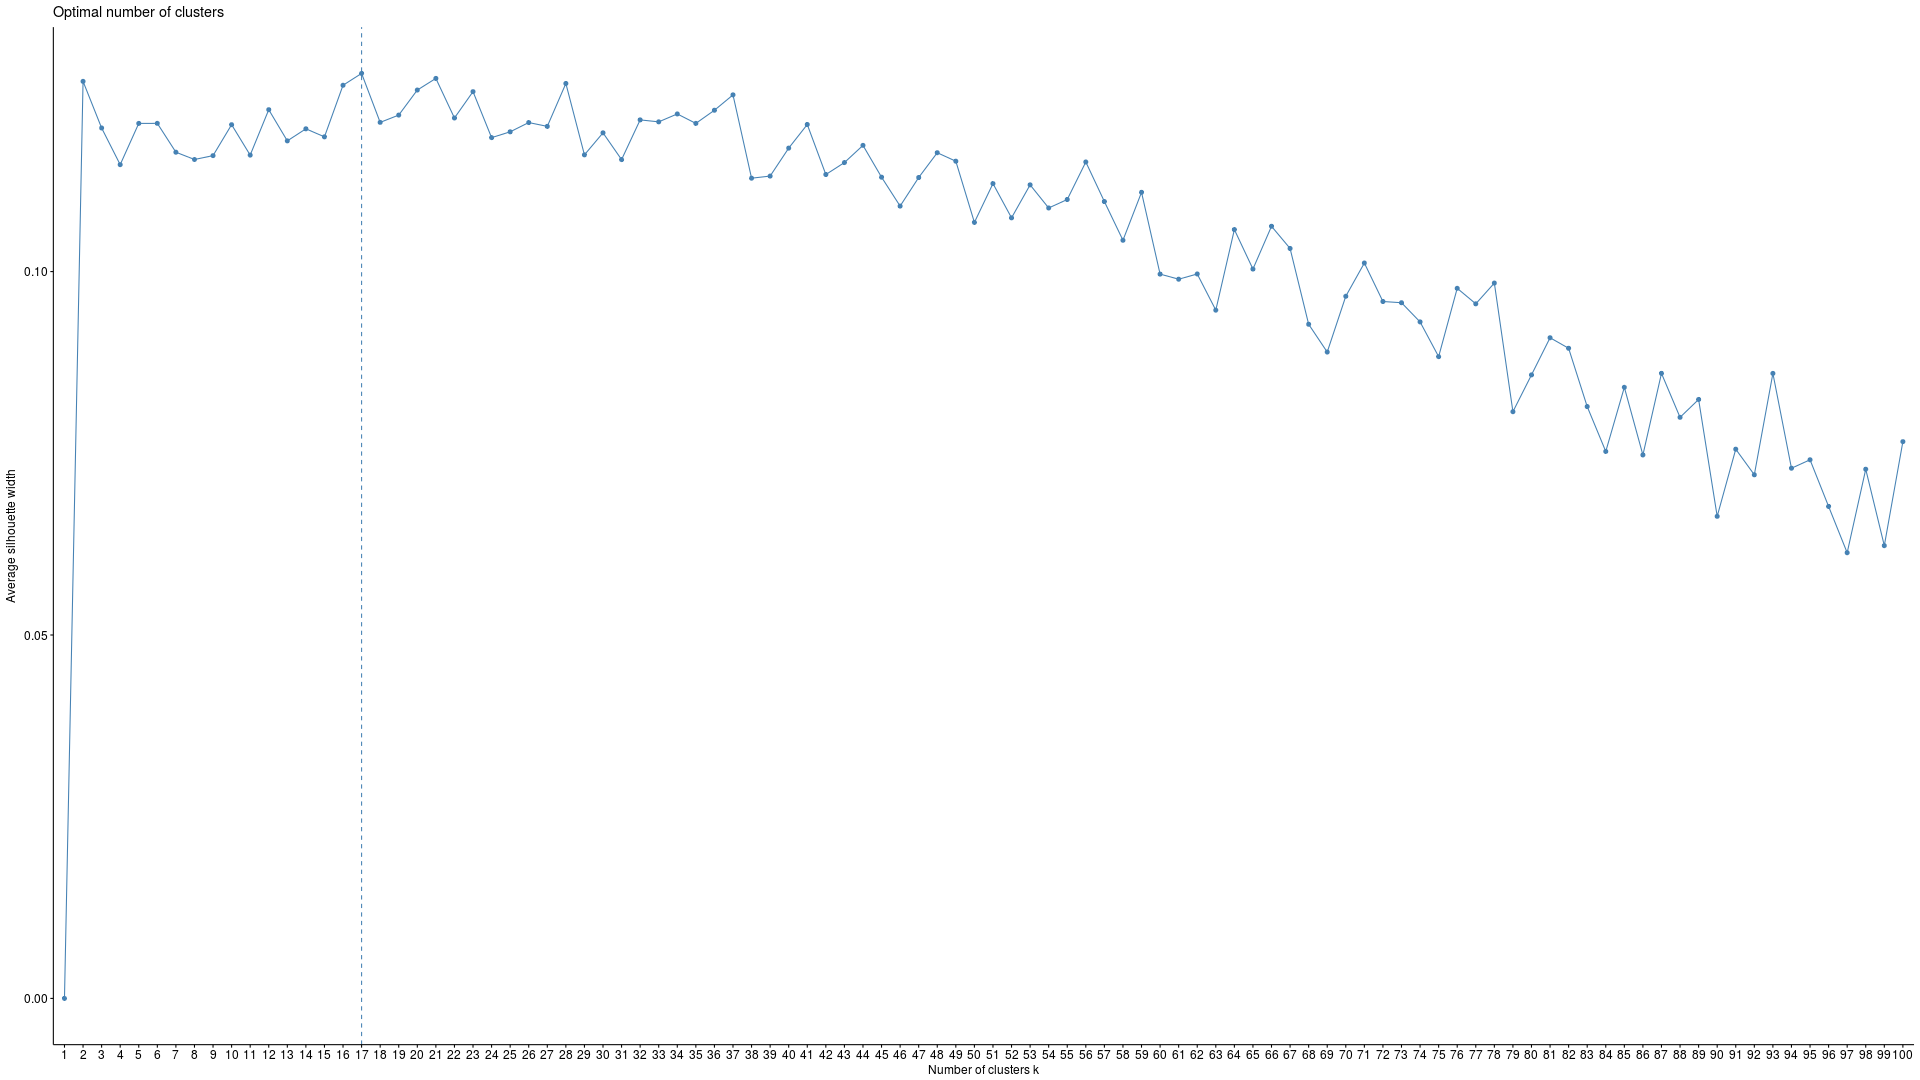
\includegraphics[width=\textwidth]{x16_sk_greyscale.png}
\caption{La largeur moyenne de la silhouette en utilisant Spherical K-means pour un intervalle de 1 \`a 100, le nombre de clust optimal est 61 pour des blocs 16x16 avec un filtre gris.} \label{fig4}
\end{figure}

\begin{figure}
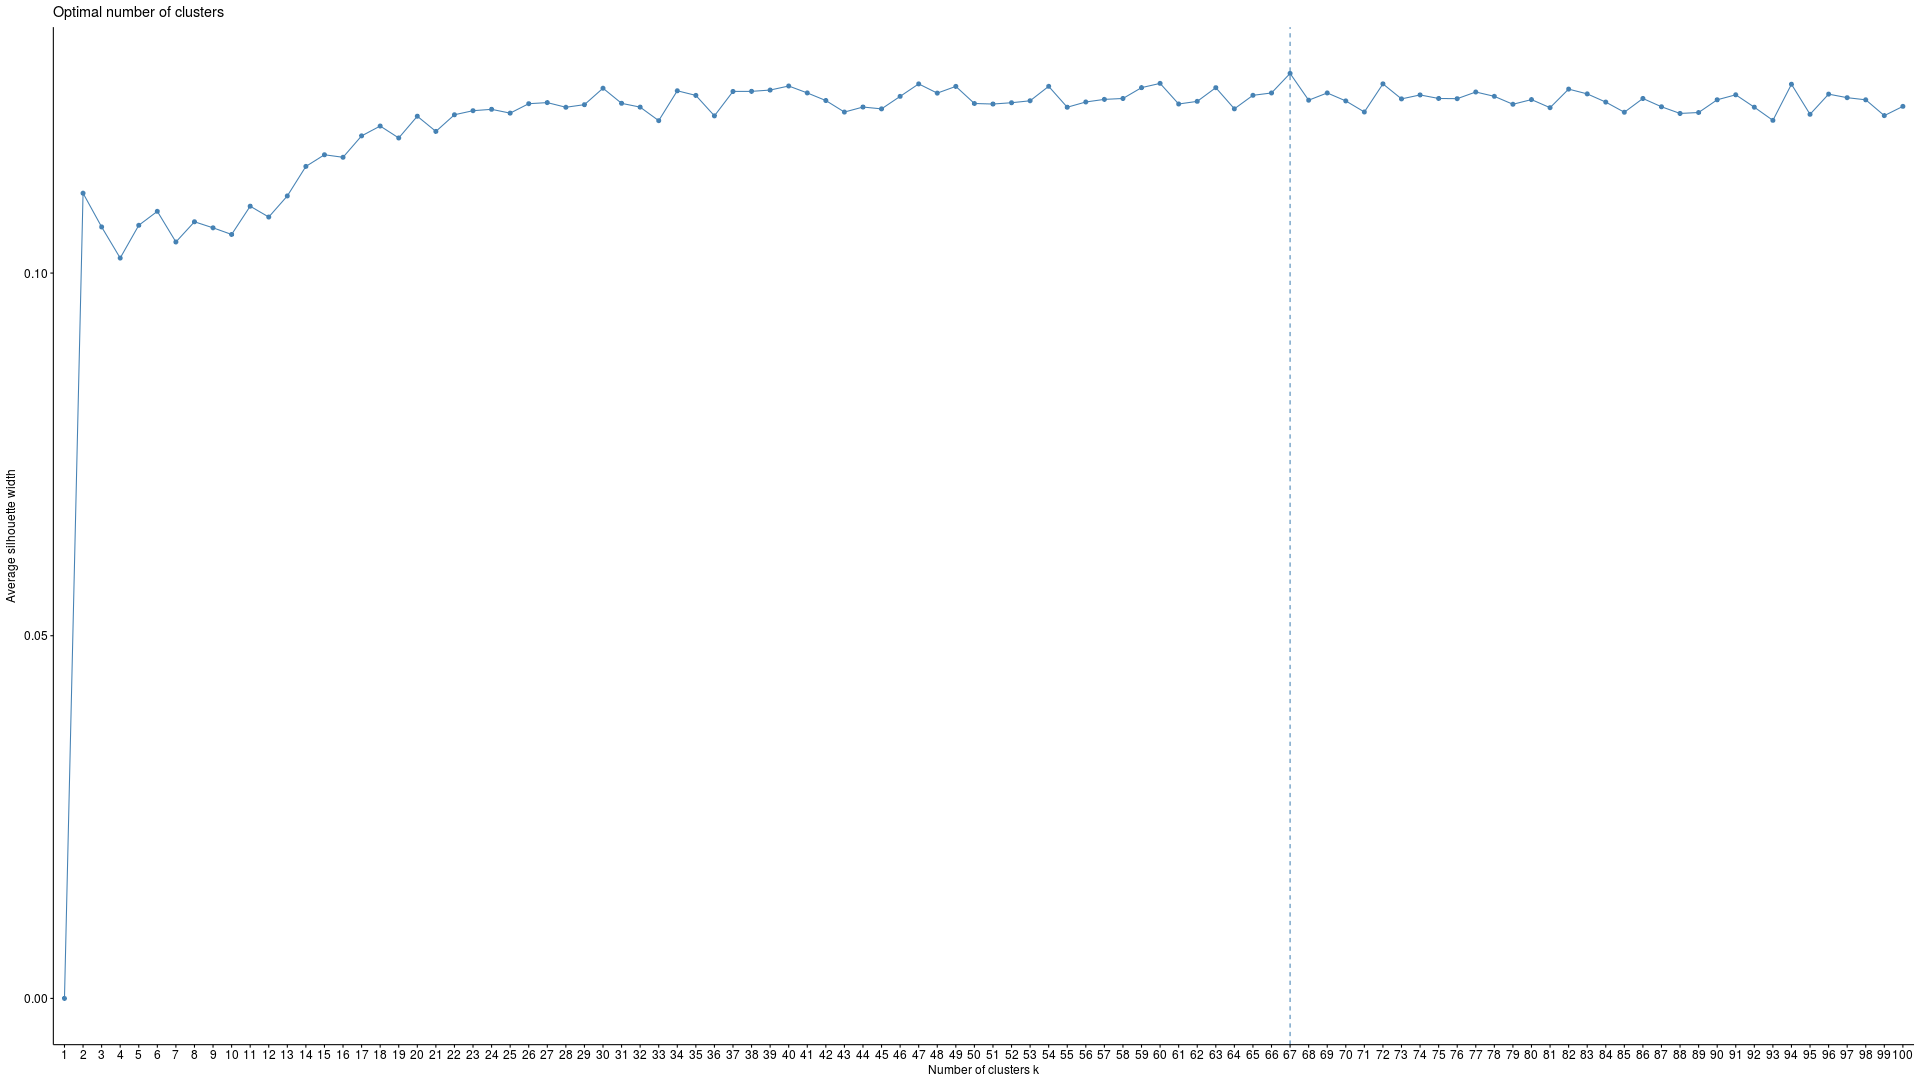
\includegraphics[width=\textwidth]{x32_sk_greyscale.png}
\caption{La largeur moyenne de la silhouette en utilisant Spherical K-means pour un intervalle de 1 \`a 100, le nombre de clust optimal est 67 pour des blocs 32x32 avec un filtre gris.} \label{fig5}
\end{figure}

\begin{figure}
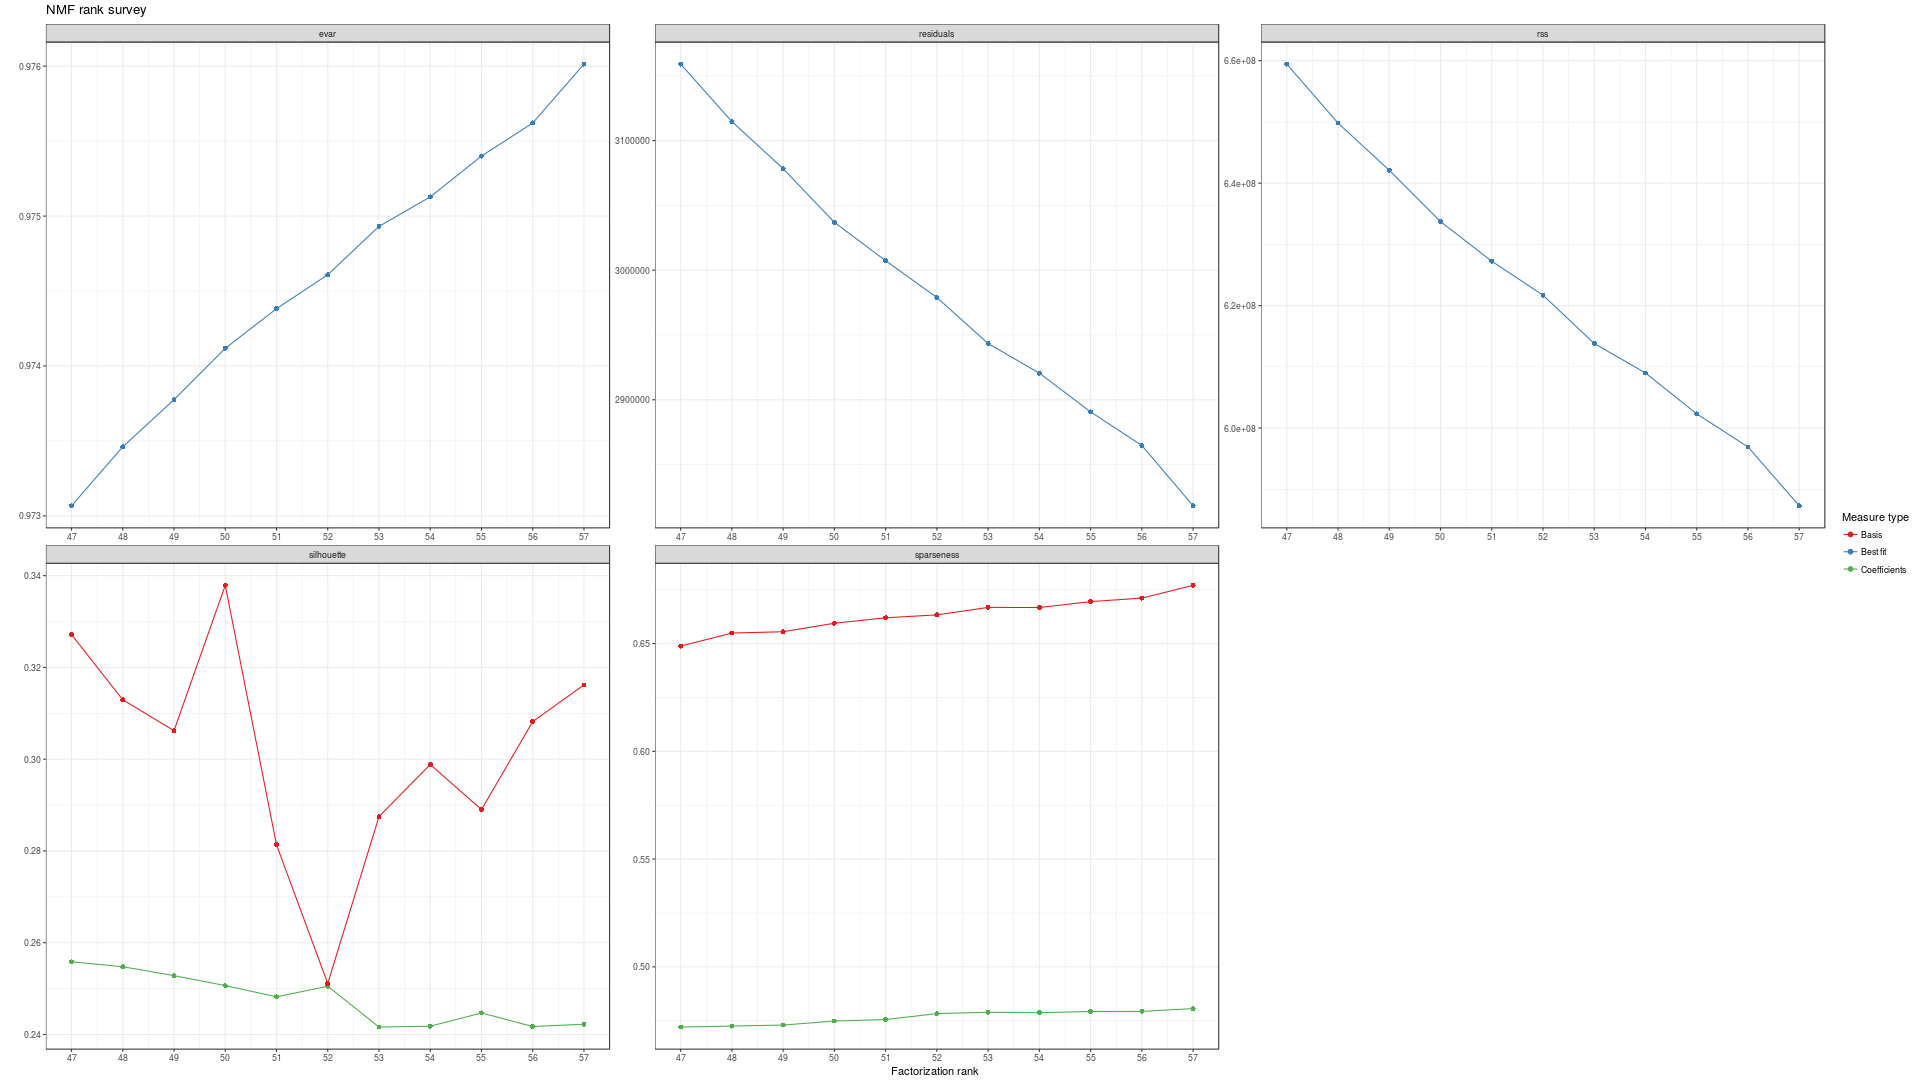
\includegraphics[width=\textwidth]{nmf-16-greyscale-47-57-KL-nndsvd.png}
\caption{Différents r\'esultats significatifs pour 16x16 avec un filtre gris, l'intervalle de 47 à 57 avec l'algorithme KL et une initialisation avec une NNDSVD.} \label{fig6}
\end{figure}

\begin{figure}
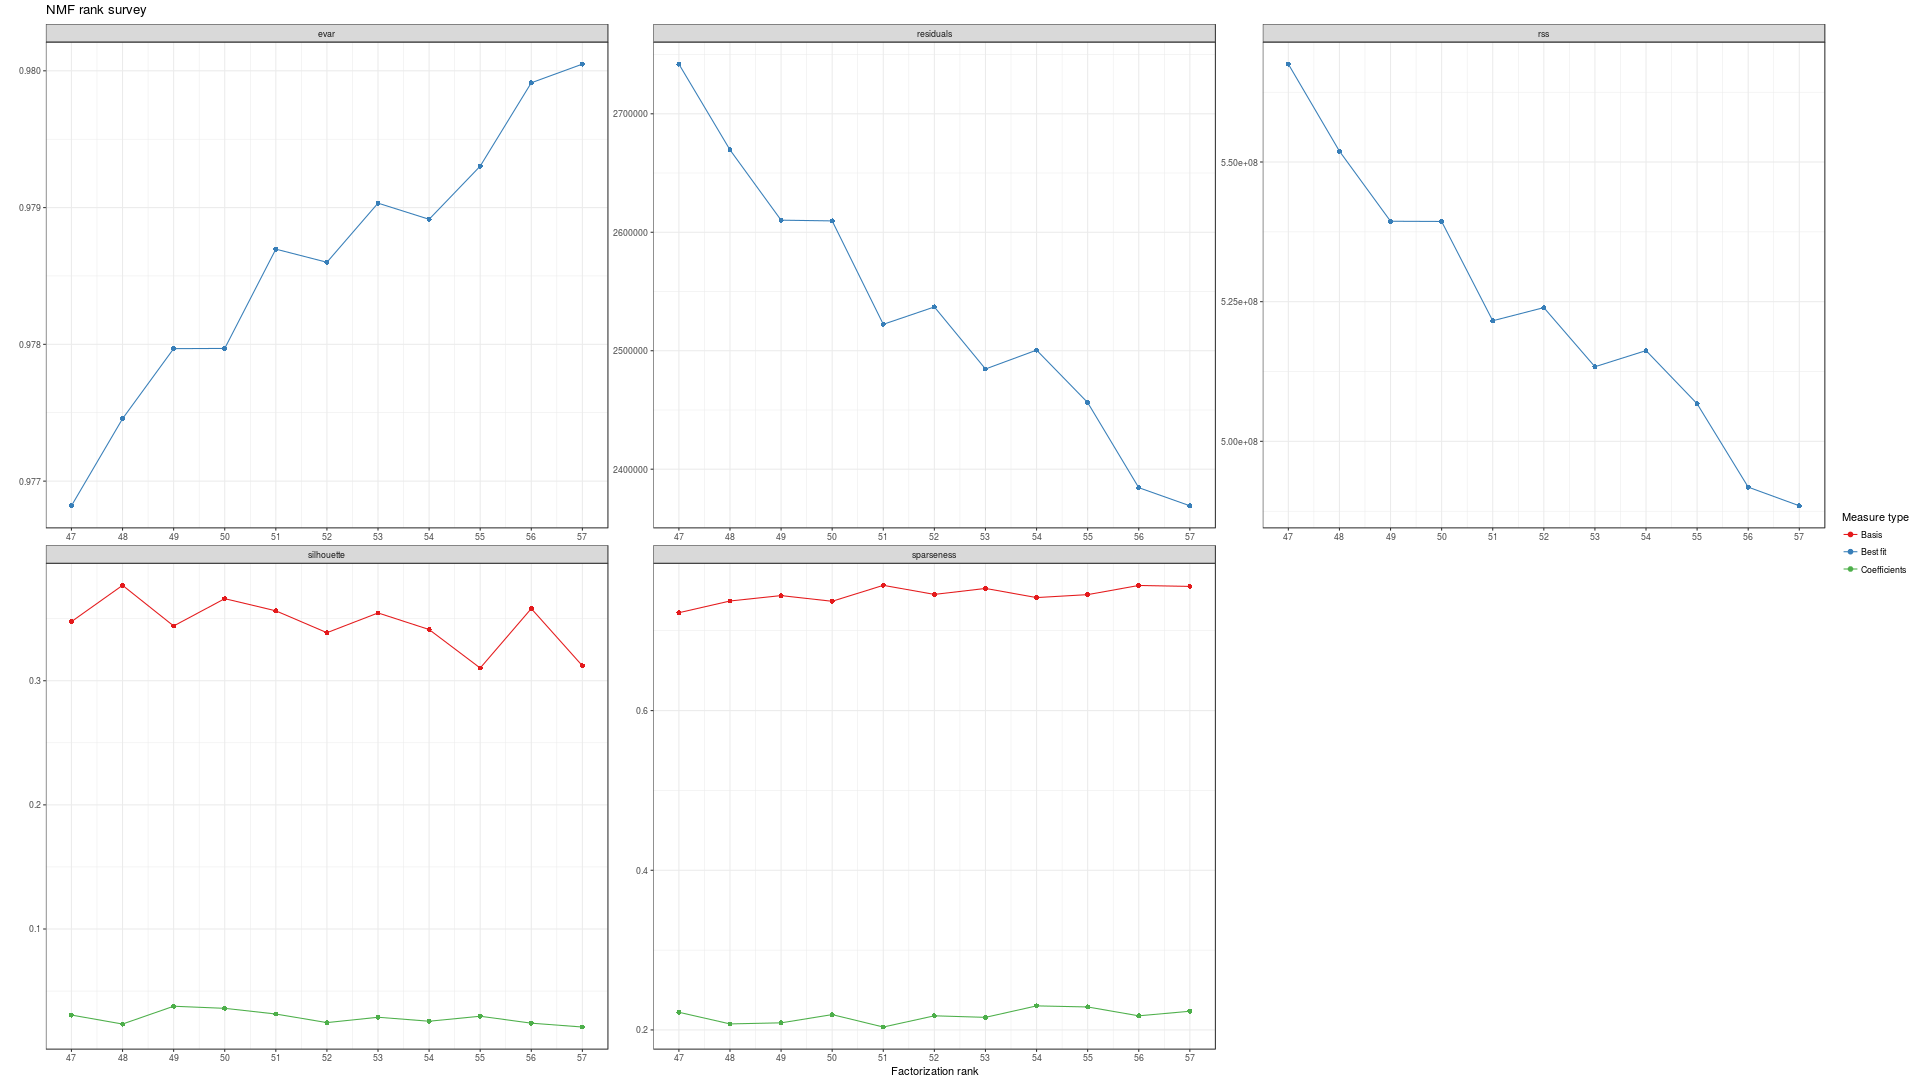
\includegraphics[width=\textwidth]{nmf-16-greyscale-47-57-KL-random.png}
\caption{Différents r\'esultats significatifs pour 16x16 avec un filtre gris, l'intervalle de 47 à 57 avec l'algorithme KL et une initialisation de manière aléatoire.} \label{fig6}
\end{figure}

\begin{figure}
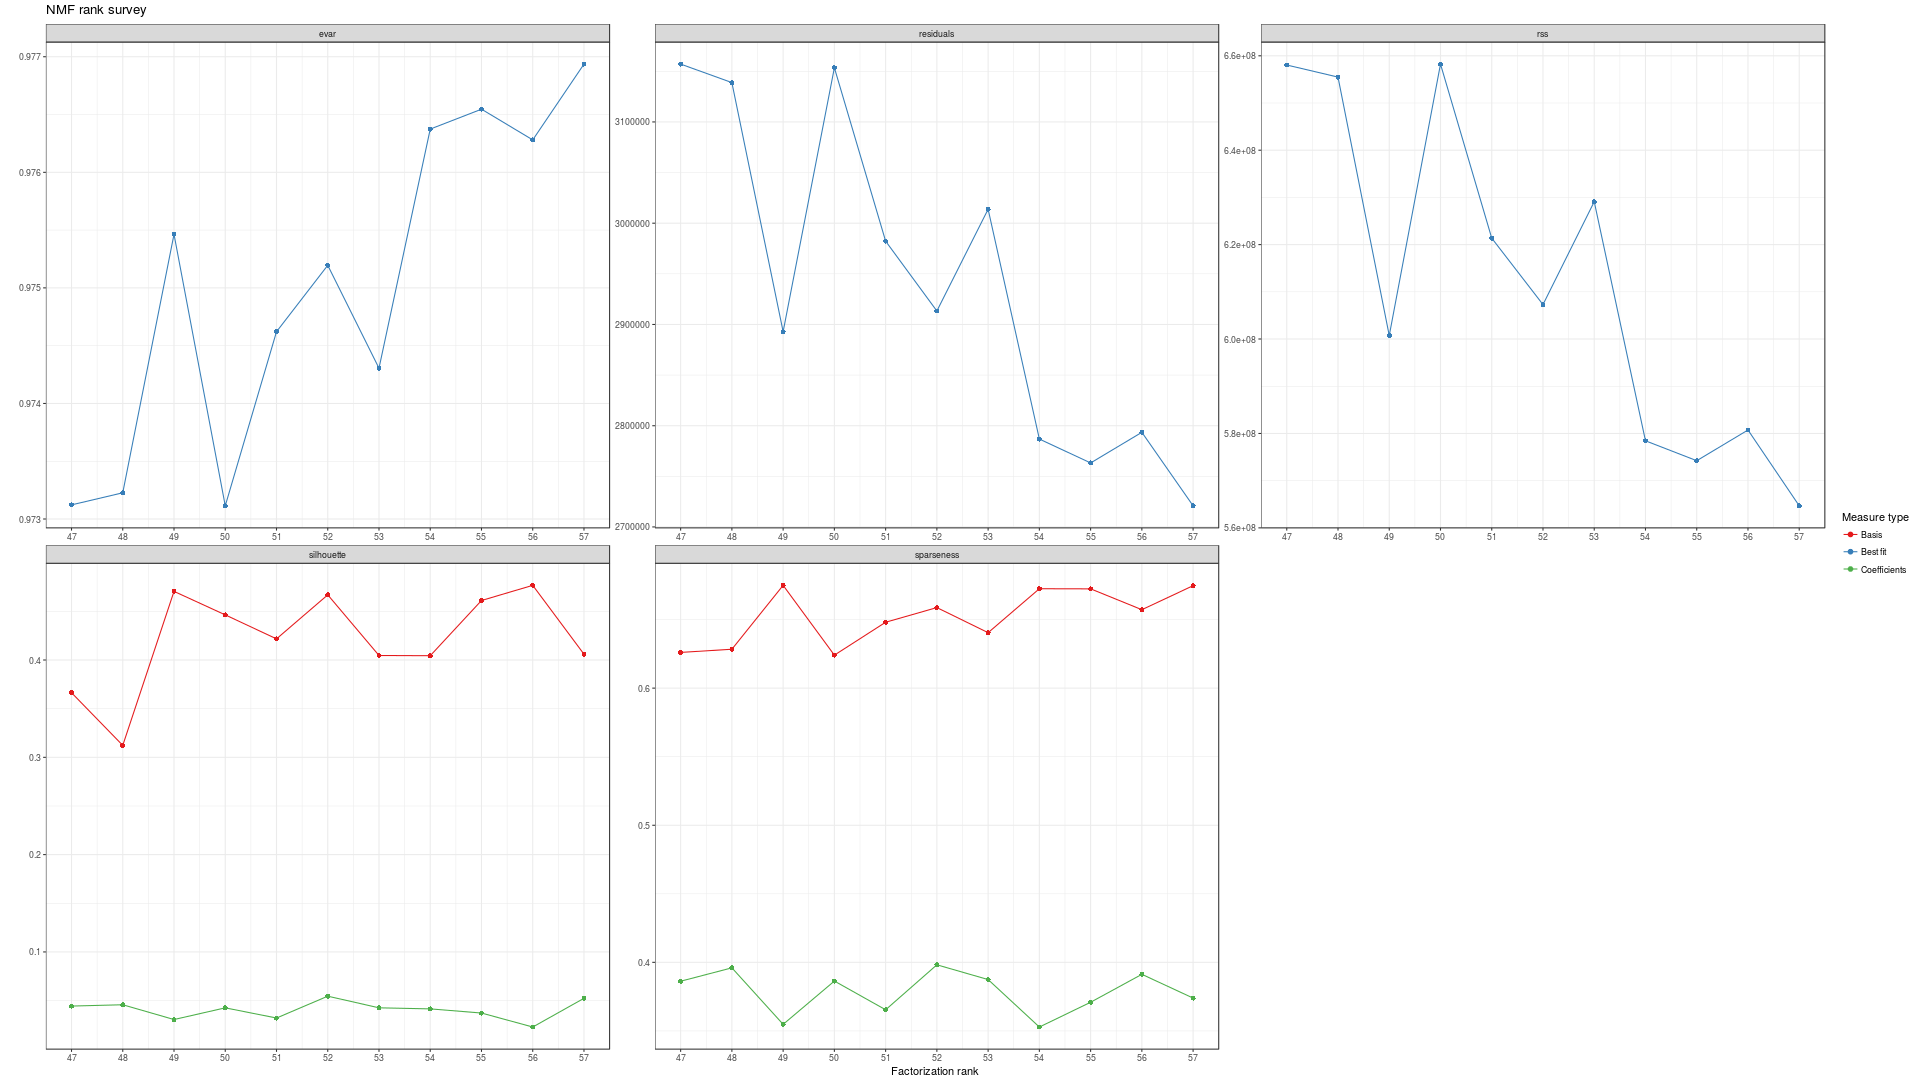
\includegraphics[width=\textwidth]{nmf-16-greyscale-47-57-KL-ica.png}
\caption{Différents r\'esultats significatifs pour 16x16 avec un filtre gris, l'intervalle de 47 à 57 avec l'algorithme KL et une initialisation avec une ICA.} \label{fig6}
\end{figure}

\begin{figure}
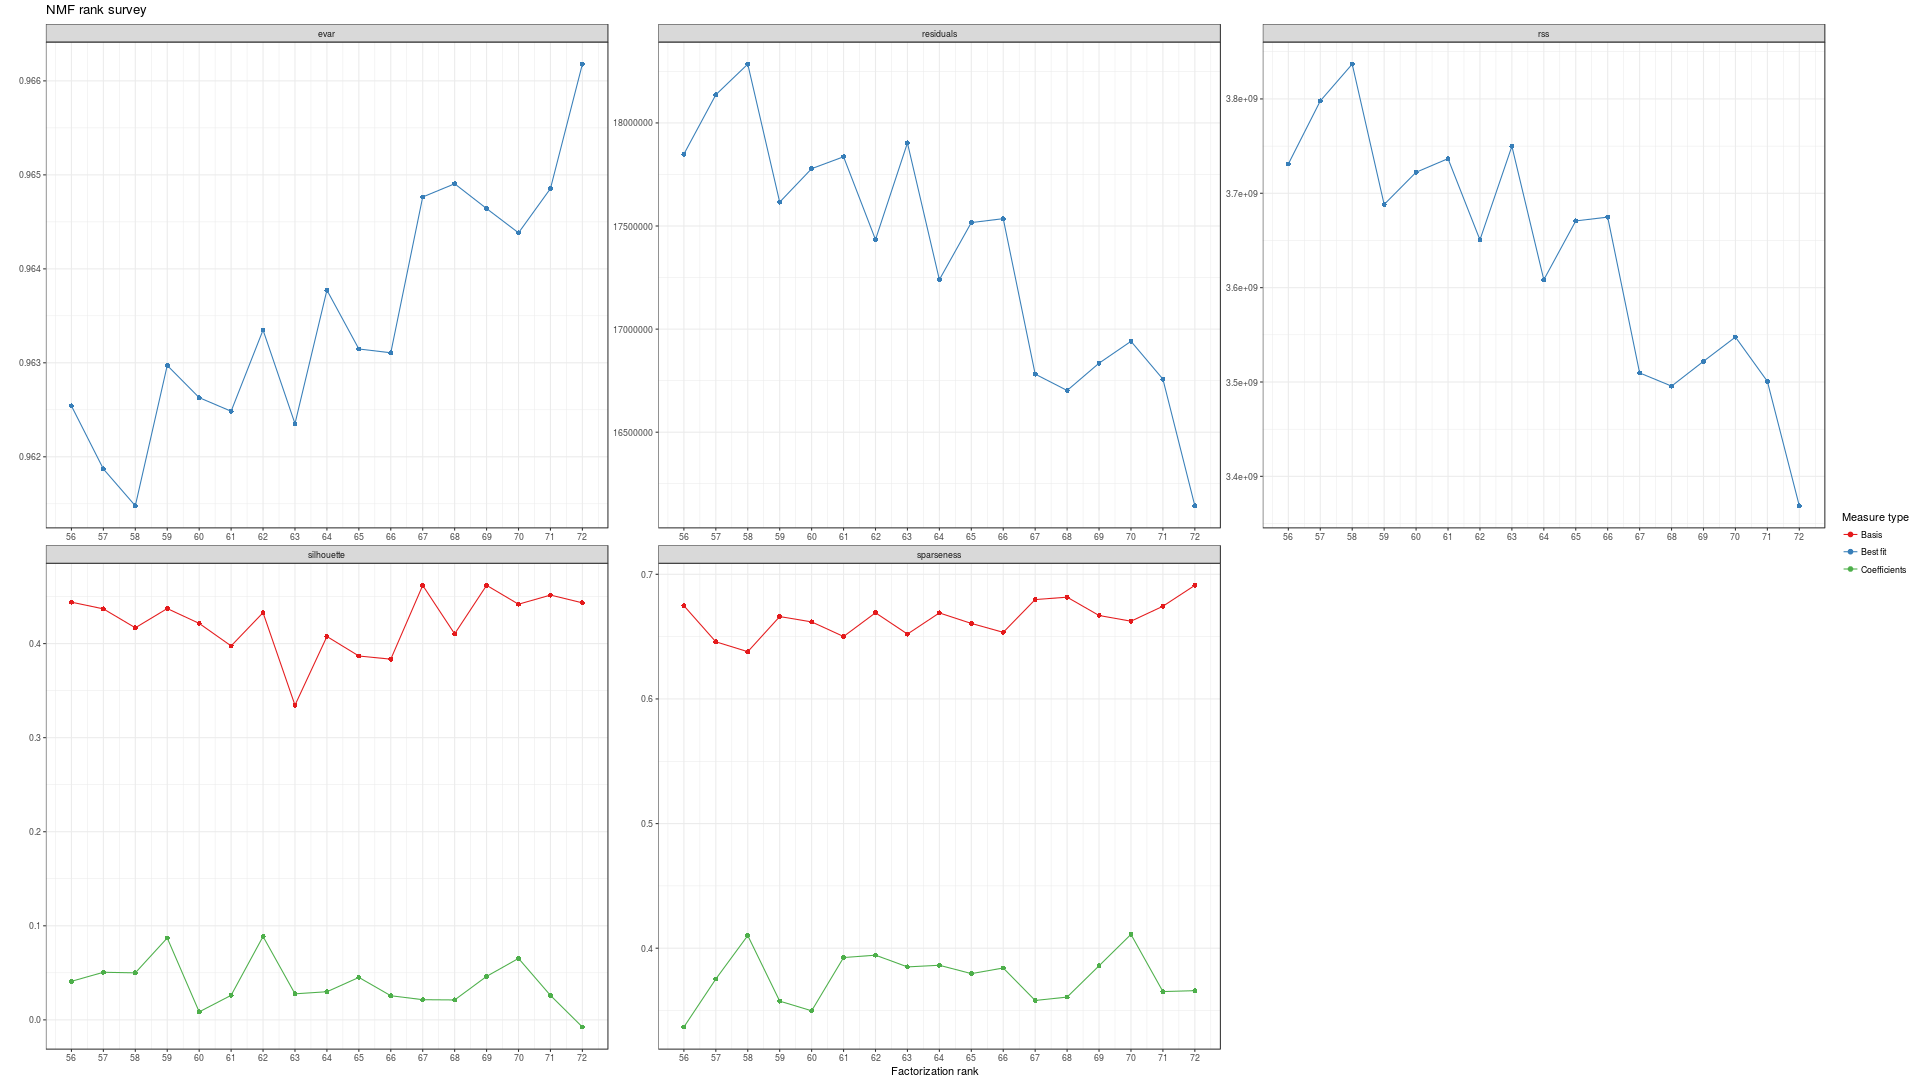
\includegraphics[width=\textwidth]{nmf-32-greyscale-56-72-KL-ica.png}
\caption{Différents r\'esultats significatifs pour 32x32 avec un filtre gris, l'intervalle de 56 à 72 avec l'algorithme KL et une initialisation avec une ICA.} \label{fig6}
\end{figure}

\begin{figure}
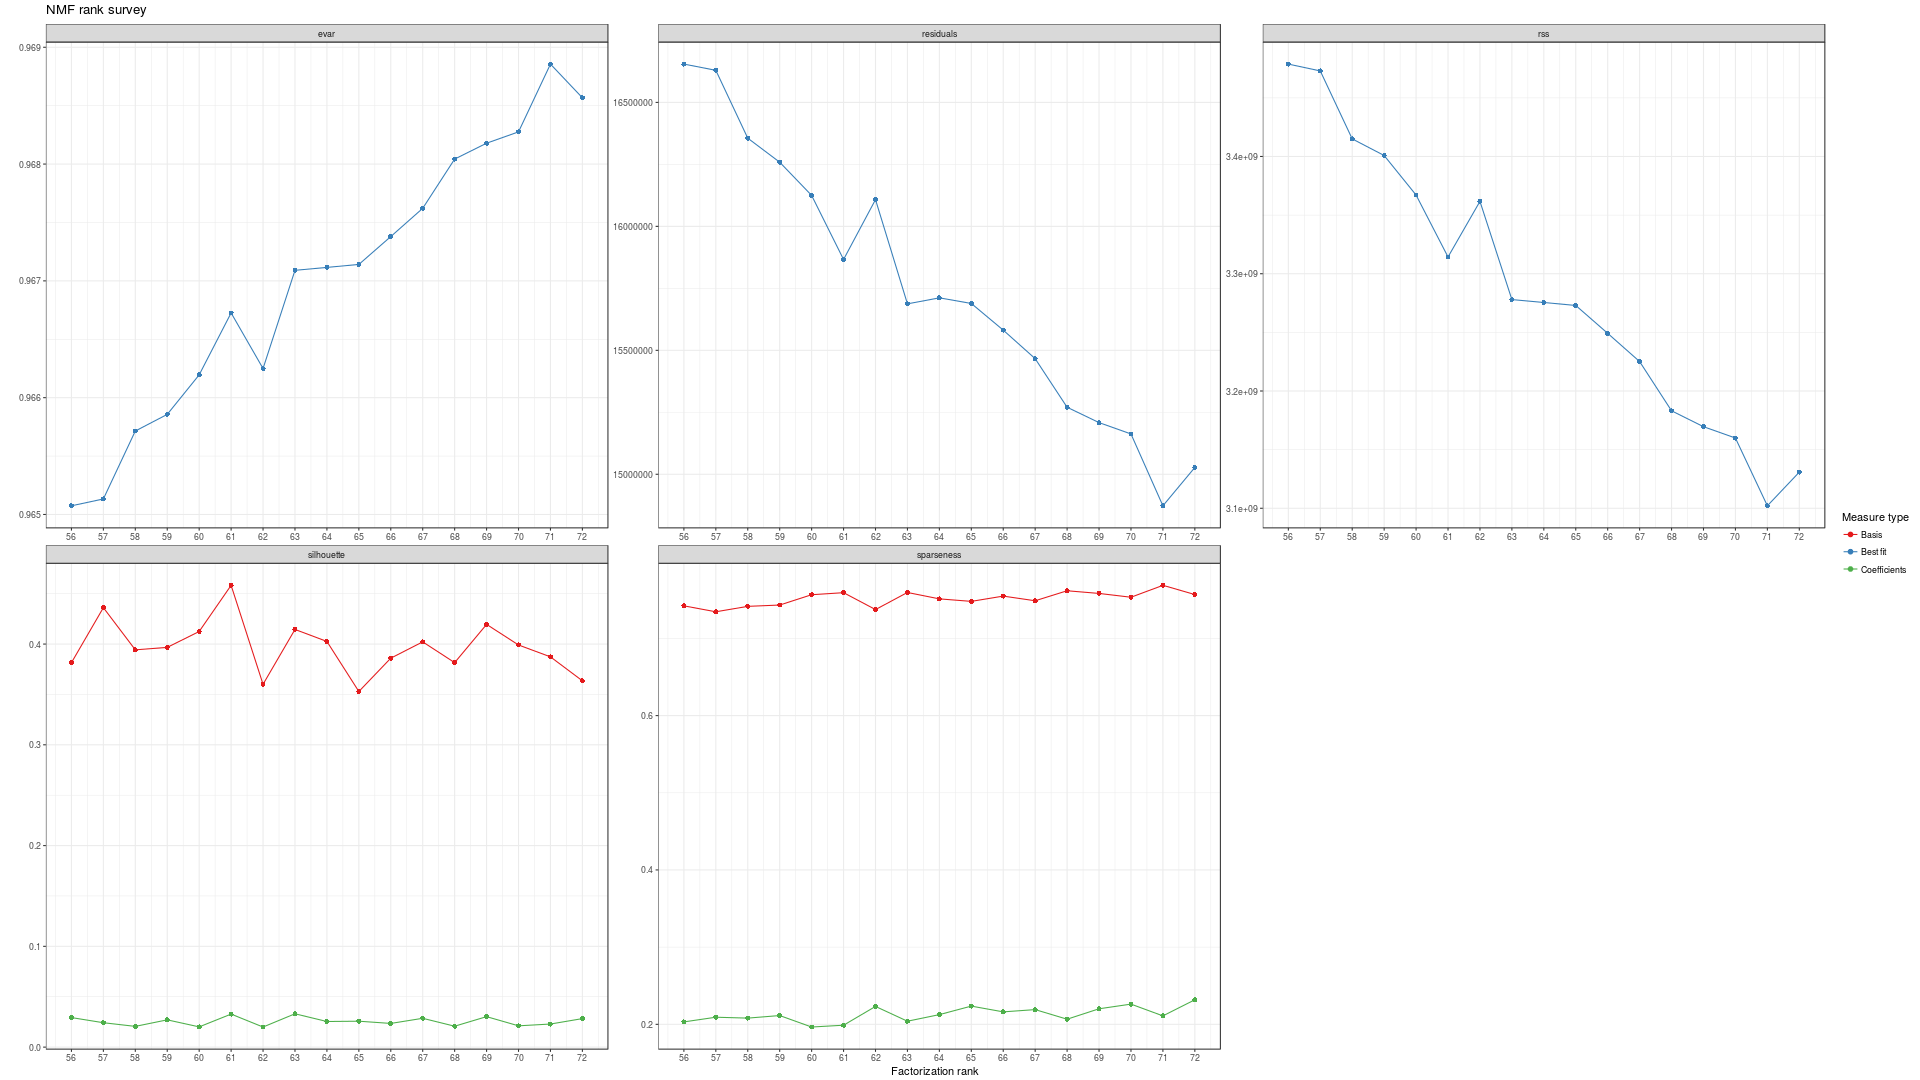
\includegraphics[width=\textwidth]{nmf-32-greyscale-56-72-KL-random.png}
\caption{Différents r\'esultats significatifs pour 32x32 avec un filtre gris, l'intervalle de 56 à 72 avec l'algorithme KL et une initialisation avec de manière aléatoire.} \label{fig6}
\end{figure}

\begin{figure}
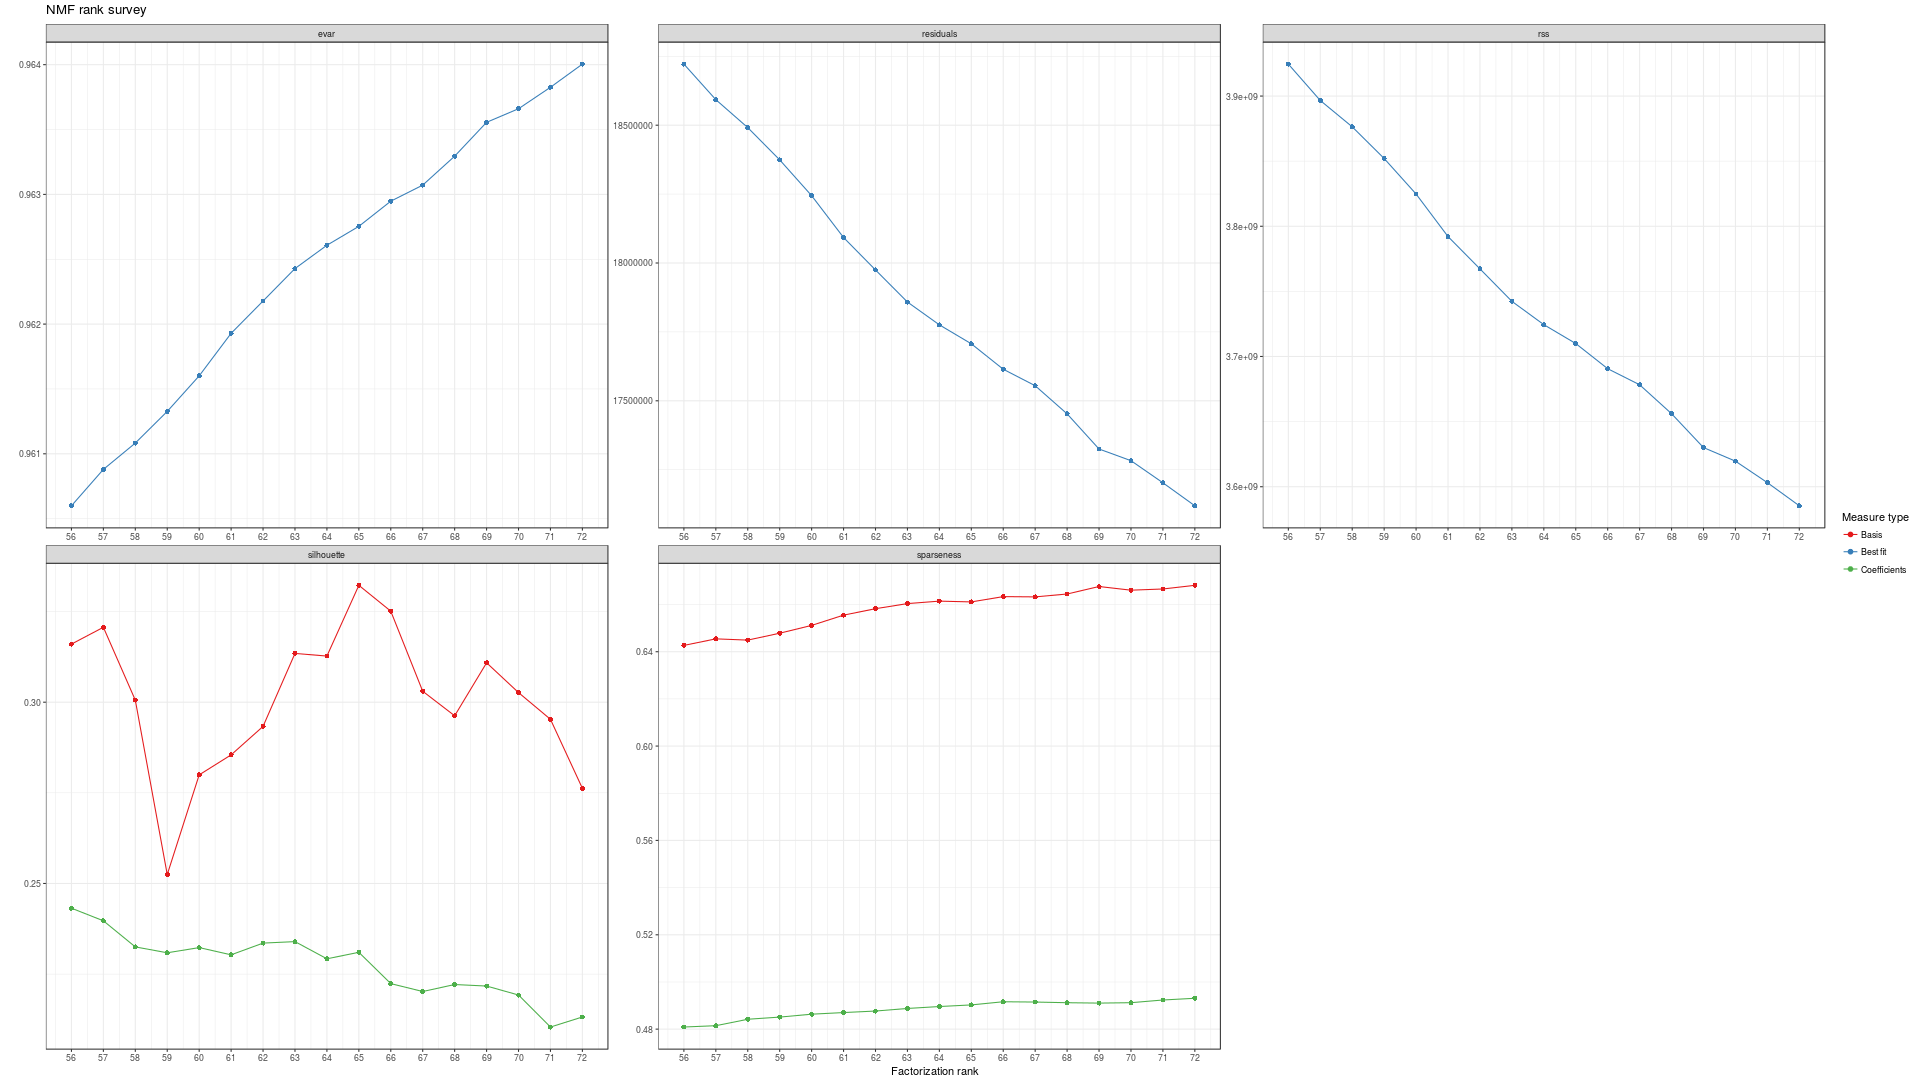
\includegraphics[width=\textwidth]{nmf-32-greyscale-56-72-KL-nndsvd.png}
\caption{Différents r\'esultats significatifs pour 32x32 avec un filtre gris, l'intervalle de 56 à 72 avec l'algorithme KL et une initialisation avec une NNDSVD.} \label{fig6}
\end{figure}


\subsubsection{Overfitting}
Even on random data, increasing the factorization rank would lead to decreasing residuals, as more variables are available to better fit the data.
In other words, there is potentially an overfitting problem. 
 
In this context, the approach from \cite{Frigyesi2008} may be useful to prevent or detect overfitting as it takes into account the results for unstructured data.
However it requires to compute the quality measure(s) for the random data.
The NMF package provides a function that shuffles the original data, by permuting the rows of each column, using each time a different permutation.
The rank estimation procedure can then be applied to the randomized data, and the random measures added to the plot for comparison.


%
% ---- Bibliography ----
%
% BibTeX users should specify bibliography style 'splncs04'.
% References will then be sorted and formatted in the correct style.
%
% \bibliographystyle{splncs04}
% \bibliography{mybibliography}
%
\begin{thebibliography}{8}
\bibitem{Brunet2004}
Author, F.: Article title. Journal \textbf{2}(5), 99--110 (2016)

\bibitem{Cichocki2008}
Author, F., Author, S.: Title of a proceedings paper. In: Editor,
F., Editor, S. (eds.) CONFERENCE 2016, LNCS, vol. 9999, pp. 1--13.
Springer, Heidelberg (2016). \doi{10.10007/1234567890}

\bibitem{Hutchins2008}
Author, F., Author, S., Author, T.: Book title. 2nd edn. Publisher,
Location (1999)

\bibitem{Frigyesi2008}
Author, A.-B.: Contribution title. In: 9th International Proceedings
on Proceedings, pp. 1--2. Publisher, Location (2010)

\bibitem{ref_url1}
LNCS Homepage, \url{http://www.springer.com/lncs}. Last accessed 4
Oct 2017
\end{thebibliography}
\end{document}